\documentclass{ctexart}

\usepackage{van-de-la-sehen}

\begin{document}

\section*{热力学} % (fold)
\label{sec:热力学}

\begin{finale}
	参考HG.1.5., 1.6., 1.7., 1.8., 1.9., 1.10., 理想气体方程为
	\[ pV = nRT \quad \Longleftrightarrow \quad p\mu = \rho RT. \]
	\[ R = \SI{8.314}{\joule\mole\per\kelvin}. \]
\end{finale}
\begin{finale}
	参考HG.1.9., 1.10., HG.2.10., 物体直接混合的温度为
	\[ T_f = \frac{m_1C_1T_1 + m_2C_2T_2}{m_1C_1+m_2C_2}. \]
\end{finale}
\begin{finale}
	参考HG.2.14.,
	\[ \pare{\ddelon{U}{*}}_{\Phi} = \pare{\frac{\dbar{Q}-p\,\rd{V}}{\partial *}}_{\Phi}. \]
\end{finale}
\begin{finale}
	参考HG.2.14,
	\[ \rd{U} = T\,\rd{S} - p\,\rd{V}. \]
\end{finale}
\begin{finale}
	参考HG.2.14., 熵的Maxwell关系,
	\[ \pare{\ddelon{S}{V}}_T = \pare{\ddelon{p}{T}}_V,\quad \pare{\ddelon{S}{p}}_T = -\pare{\ddelon{V}{T}}_p. \]
	两条对角线分别是$ST$和$pV$, 约束相应为另一侧的偏微分变量.
\end{finale}
\begin{finale}
	参考HG.2.14., 2.16., 2.18., 2.19.,
	\[ C_p - C_V = T\pare{\ddelon{p}{T}}_V\pare{\ddelon{V}{T}}_p. \]
	特别地, 对理想气体,
	\[ C_p - C_V = R. \]
\end{finale}
\begin{finale}
	参考HG.3.4.
	\[ \pare{\ddelon{U}{V}}_T = T\pare{\ddelon{p}{T}}_V - p, \]
	\[ \pare{\ddelon{H}{p}}_T = -T\pare{\ddelon{V}{T}}_p + V. \]
\end{finale}
\begin{finale}
	参考HG.2.28,. 2.30., 3.3., J-T系数:
	\[ \alpha_i = \pare{\ddelon{T}{p}}_{H} = -\rec{C_p}\brac{V-T\pare{\ddelon{V}{T}}_p}. \]
	最大反转温度和最大反转压强为
	\[ T=\frac{2a}{bR},\quad p=\frac{a}{3b^2}. \]
\end{finale}
\begin{reflex}
	{$U$的偏微分恒等式的证明}{$U$的偏微分恒等式的证明} 参考HG.2.14., 2.15., 从$\rd U = \rd{Q} - p\,\rd{V}$出发, 通常将$U$参数化为$U\pare{T,V}$, 必要时使用Maxwell关系.
\end{reflex}
\begin{finale}
	参考HG.2.17., $\Delta H$即等压过程的吸热量.
\end{finale}

\begin{finale}
	参考HG.3.1., 3.10., 3.18., 对于Carnot热机,
	\[ \eta = \frac{W}{Q_{\text{endo}}} = \frac{Q_{\text{endo}} - Q_{\text{exdo}}}{Q_{\text{endo}}} = 1-\frac{T_{\text{low}}}{T_{\text{high}}}. \]
	参考HG.2.35, 制冷系数$\epsilon$谓
	\[ \epsilon = \frac{Q_{\text{endo}}}{W} = \frac{Q_{\text{endo}}}{Q_{\text{exdo}}-Q_{\text{endo}}}. \]
	效率或制冷系数总是按照「收益」/「消耗」定义.
\end{finale}
\begin{finale}
	参考D.2.3., 2.4., D.2.5., 热容相等的热源之间的Carnot热机的平衡温度
	\[ T_f = \sqrt{T_1 T_2}. \]
\end{finale}
\begin{finale}
	参考HG.3.8., 对理想气体无条件成立
	\[ \Delta U = C_V \Delta T. \]
\end{finale}
\begin{finale}
	参考HG.2.3., 2.4., 2.16., 对vdW气体, 成立
	\[ \pare{p+\frac{n^2 a}{V^2}}\pare{V-nb} = nRT. \]
	全微分有
	\[ \pare{V-nb}\,\rd{p} + f\pare{p,V}\,\rd{V} = nR\,\rd{T}. \]
\end{finale}
\begin{finale}
	$\SI{1}{mol}$vdW气体之内能为
	\[ U = C_V T - \frac{a}{V}. \]
\end{finale}
\begin{finale}
	参考HG.2.5., D.2.27., $\Delta W$即为$p$-$V$图线围成面积, 即
	\[ \Delta W = -\int_1^2 p\,\rd{V}. \]
	对于热机循环, 也恰好是$T$-$S$图线围成面积.
\end{finale}
\begin{finale}
	参考HG.1.11., 1.12., 1.13., 2.7., 对于固体,
	\[ \alpha = \rec{V}\pare{\ddelon{V}{T}}_p,\quad \beta = -\rec{V}\pare{\ddelon{V}{p}}_T. \]
	通常$\alpha, \beta>0$, 假定为常数, 固定$p$, $T$中一个后积分有
	\[ \begin{array}{cc}
		V\pare{T} = V_0 e^{\alpha T} &  V\pare{p} = V_0e^{-\beta p} \\
		\Updownarrow  & \Updownarrow \\
		T = \rec{\alpha}\ln \frac{V}{V_0} & p = -\rec{\beta}\ln \frac{V}{V_0}.
	\end{array}. \]
	线性近似有状态方程
	\[ V = V_0\brac{1+\alpha\pare{T-T_0}-\beta\pare{p-p_0}}. \]
\end{finale}
\begin{pitfall}
	参考HG.1.11, 1.12., 1.13., 状态方程通常不可直接线性近似.
\end{pitfall}
\begin{finale}
	参考HG.2.8., 有裂缝的容器, 其加热吸热量按照$C_V$计算.
\end{finale}
\begin{reflex}
	{过程方程与热容关系}{过程方程与热容关系} 参考HG.2.21., 2.22., 2.23., 2.24., 求过程方程与热容关系时, 考虑
	\[ \rd{U} = C_V\,\rd{T} = C\,\rd{T} - p\,\rd{V}, \]
	再联立状态方程, 例如$pV=nRT$或vdW方程消去$p$, 可得
	\[ \pare{C_V-C}\,\rd{T} = f\pare{T,V}\,\rd{V}, \]
	求得状态方程.
\end{reflex}

\newcolumntype{A}{>{\columncolor{MLG}}c}

\begin{table}[ht]
	\centering
	\begin{tabular}{!{\vrule width 1.5pt}A|A|A|A|A!{\vrule width 1.5pt}}
		\noalign{\hrule height 1.5pt}
		\multicolumn{5}{!{\vrule width 1.5pt}A!{\vrule width 1.5pt}}{参考HG.2.1., 2.2., 2.6., 2.18., 2.19., 2.20., 2.21., 2.25., 2.26., }\\
		\multicolumn{5}{!{\vrule width 1.5pt}A!{\vrule width 1.5pt}}{2.27., 3.8., 3.9., }\\
		\hline
		名称 & 约束 & $\Delta W$ & $\Delta Q$ & 摩尔热容 \\
		\hline
		& $V=\const$ & & & \\
		\multirow{-2}{*}{定体} & $p/T = \const$ & \multirow{-2}{*}{$0$} & \multirow{-2}{*}{$C_V\Delta T$} & \multirow{-2}{*}{$\displaystyle C_V=\frac{R}{\gamma-1}$} \\
		\hline
		& $p=\const$ & $-p\Delta V$ & & \\
		\multirow{-2}{*}{定压} & $T/V=\const$ & $-\nu R\Delta T$ & \multirow{-2}{*}{$C_p\Delta T$} & \multirow{-2}{*}{$\displaystyle C_p = \frac{\gamma R}{\gamma-1}$} \\
		\hline
		 & & & & \\
		& \multirow{-2}{*}{$T=\const$} & \multirow{-2}{*}{$\displaystyle -p_1V_1 \ln \frac{V_2}{V_1}$} & \multirow{-2}{*}{$\displaystyle p_1V_1\ln \frac{V_2}{V_1}$} & \\
		& & & & \\
		\multirow{-4}{*}{等温} & \multirow{-2}{*}{$pV=\const$} & \multirow{-2}{*}{$\displaystyle -\nu RT\ln \frac{V_2}{V_1}$} & \multirow{-2}{*}{$\displaystyle \nu RT_1\ln \frac{V_2}{V_1}$} & \multirow{-4}{*}{$\infty$} \\
		\hline
		& $pV^\gamma=\const$  & & & \\
		& $TV^{\gamma-1}=\const$ & \multirow{-2}{*}{$\displaystyle \frac{\Delta\pare{pV}}{\gamma-1}$} & & \\
		& & & & \\
		\multirow{-4}{*}{绝热} & \multirow{-2}{*}{$\displaystyle \frac{T^\gamma}{p^{\gamma-1}} = \const$} & \multirow{-2}{*}{$C_V\Delta T$} & \multirow{-4}{*}{$0$} & \multirow{-4}{*}{$0$} \\
		\hline
		& $pV^n=\const$ & & & \\
		& $TV^{n-1}=\const$ & \multirow{-2}{*}{$\displaystyle \frac{\Delta\pare{pV}}{n-1}$} & & \multirow{-2}{*}{$\displaystyle C_n = C_V - \frac{R}{n-1}$} \\
		& & & & \\
		\multirow{-4}{*}{多方} & \multirow{-2}{*}{$\displaystyle \frac{T^n}{p^{n-1}} = \const$} & \multirow{-2}{*}{$\displaystyle \frac{\nu R}{n-1}\Delta T$} & \multirow{-4}{*}{$C_n\Delta T$} & \multirow{-2}{*}{$\displaystyle \phantom{C_n} = C_V\cdot\frac{\gamma-n}{1-n}$} \\
		\noalign{\hrule height 1.5pt}
	\end{tabular}
\end{table}

\begin{reflex}
	{热机效率的计算}{热机效率的计算} 参考HG.2.31., 2.32., 2.34., 2.35., 2.36., 计算热机/制冷效率时, 划分吸热与放热过程, 分别写出其$Q$值.
\end{reflex}
\begin{pitfall}
	参考HG.2.35., 2.36., 与环境的热量交换最终需忽略.
\end{pitfall}
\begin{finale}
	参考HG.2.34., Carnot循环由等温和绝热过程构成. $p$-$V$图上绝热过程的线斜率较大.
\end{finale}
\begin{finale}
	参考D.1.25., 1.35., 容器泄气过程之气体做功视为对抗「可活动部分」之压强之做功. 于气体快速进入容器的情形下亦然.
\end{finale}
\begin{pitfall}
	参考D.1.24., 1.25., 非平衡过程即使在绝热容器内亦不可使用$\cancel{pV^\gamma=\const.}$.
\end{pitfall}
\begin{finale}
	参考HG.3.5., 3.13., 3.14., 3.18.,
	\[ \rd{Q}_{\mathrm{rev}} = T\,\rd{S},\quad \pare{\ddelon{S}{\ln T}}_V = C_V. \]
\end{finale}
\begin{finale}
	参考HG.3.5., 内能密度
	\[ u = \frac{U}{V} = \frac{C_V}{R}p. \]
\end{finale}

\begin{reflex}
	{过程中热学量的不等式的证明}{过程中热学量的不等式的证明} 参考HG.3.10., 3.11., D.2.13., 从Clausius不等式$\Delta S\ge 0$出发, 将热力学量与$S$关联.
\end{reflex}

\begin{finale}
	参考HG.3.7., 3.8., 3.9., 3.12., 3.16., 3.17., D.2.14.,
	\begin{align*}
		\Delta S &= C_V \ln\frac{T_2}{T_1} + \nu R\ln\frac{V_2}{V_1} \\
		&= C_p \ln\frac{T_2}{T_1} - \nu R\ln\frac{p_2}{p_1}.
	\end{align*}
\end{finale}

\begin{finale}
	参考HG.3.11, D.2.28., 2.29., 2.30., 对于孤立系统总有
	\[ \Delta S \ge 0. \]
	特别地, 对于可逆热机(具有最大工作效率)总有$\Delta S = 0$.
\end{finale}
\begin{finale}
	参考TSZY.1.7., 无论是否可逆的循环皆成立
	\[ \oint \frac{\rd{Q}}{T} \le 0. \]
\end{finale}
\begin{finale}
	参考HG.3.15., 混合气体的熵:
	\[ \Delta S = \sum \nu_i R\ln \frac{V}{V_i}. \]
\end{finale}

\begin{reflex}
	{过程中热学量的等式的证明}{过程中热学量的等式的证明} 参考HG.2.11., 先构造容易计算的(准静态)可逆过程.
\end{reflex}

\begin{finale}
	\centerline{
		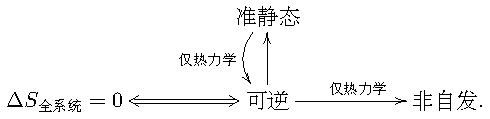
\includegraphics{src/relations.pdf}
	}
	非热力学的情形下, 有摩擦的准静态过程不可逆, 且自发的力学过程可以可逆.
\end{finale}

% section 热力学 (end)

\end{document}
